%includo tutti i pacchetti necessari e setto alcune impostazioni
\documentclass[a4paper]{article}
\usepackage[T1]{fontenc}
\usepackage[utf8]{inputenc}
\usepackage[english,italian]{babel}
\usepackage{graphicx}
\usepackage[a4paper,top=3cm,bottom=3cm,left=3cm,right=3cm]{geometry} 
\usepackage[fontsize=13pt]{scrextend}
\usepackage{fancyhdr}
\raggedbottom

%--------------------------------------------------------------------------%

\begin{document}

%aggiungo il frontespizio
\input{frontespizio}

\pagestyle{fancy}

\fancyhead{}
\fancyhead[R]{IL PAROLIERE ONLINE}

\fancyfoot{} 
\fancyfoot[L]{Giulio Bartoloni}
\fancyfoot[C]{\thepage}
\fancyfoot[R]{Matricola 654370}

%--------------------------------------------------------------------------%

\tableofcontents
\newpage
    \section{Istruzioni per la compilazione ed esecuzione}
    All'interno del file .zip di consegna si può trovare il \textbf{Makefile}, contenente tutte le regole necessarie per la corretta compilazione del progetto:
    \begin{itemize}
        \item \textbf{make (all)}: target di default, permette di compilare sia il client che il server insieme a tutti i file di libreria necessari per entrambi.
        \item \textbf{make server}: il comando permette di compilare solo i file necessari al server.
        \item \textbf{make client}: il comando permette di compilare solo i file necessari al client.
        \item \textbf{cleanall}: verranno rimossi tutti i risultati della compilazione, lasciando solo i file sorgente.
        \item \textbf{cleanserver}: rimuove tutto quello che il comando \textbf{make server} crea.
        \item \textbf{cleanclient} rimuove tutto quello che il comando \textbf{make client} crea.
    \end{itemize}
    
    Per quanto riguarda l'esecuzione del codice, questa rispetta le specifiche della consegna:
    \begin{itemize}
         \item \textbf{./paroliere\_srv nome\_server porta\_server} con i parametri opzionali \textbf{[--matrici\ data\_filename]} \textbf{[--durata\ durata\_gioco\_in\_minuti]}
         \textbf{[--seed\ rnd\_seed]} \textbf{[--diz\ dizionario]}
         \\I parametri opzionali possono essere utilizzati in qualunque ordine. L'unica regola è che i parametri \textbf{--seed} e \textbf{--matrici} non possono essere utilizzati contemporaneamente.
         \item \textbf{./paroliere\_srv nome\_server porta\_server}
    \end{itemize}

    
    
    \section{Organizzazione del codice}
    Data la complessità del progetto, ho sviluppato il codice in modo modulare, dividendo il lavoro in blocchi logicamente separati. Questo approccio mi ha spinto quindi a separare il codice in diverse librerie, migliorando notevolmente la modularità e facilitando il riutilizzo delle funzioni anche all'esterno del progetto. Ognuna di queste librerie contiene funzioni cruciali sia per evitare ridondanza nel codice, che per facilitarne la lettura permettendo una migliore comprensione. 
    
    Sia il server che il client dispongono di librerie "personali" contenenti funzioni e/o struct specifiche per essi, ma c'è anche una libreria di funzioni condivise (\textbf{'shared\_functions.c'}) e un file di macros (\textbf{'macros.h'}) con alcune utilities per entrambi. Le librerie sono tutte compilate e linkate attraverso il Makefile per garantire che sia il server che il client abbiano accesso a tutto il necessario. 
    
    Poiché alcune di queste funzioni richiedevano accesso in maniera specifica ad alcune variabili dichiarate nei due file principali, ho deciso di spostarle in questi ultimi per evitare una lista di parametri eccessivamente lunga e un conseguente peggioramento nella chiarezza del codice.


    
    \section{Struttura dei programmi}
    Il progetto è suddiviso nei due file \textbf{paroliere\_srv.c} e \textbf{paroliere\_cl.c}. Per entrambi ho adottato un approccio multithreaded al fine di garantire il comportamento richiesto e buone prestazioni.
    \begin{figure}[!htb]
        \centering
        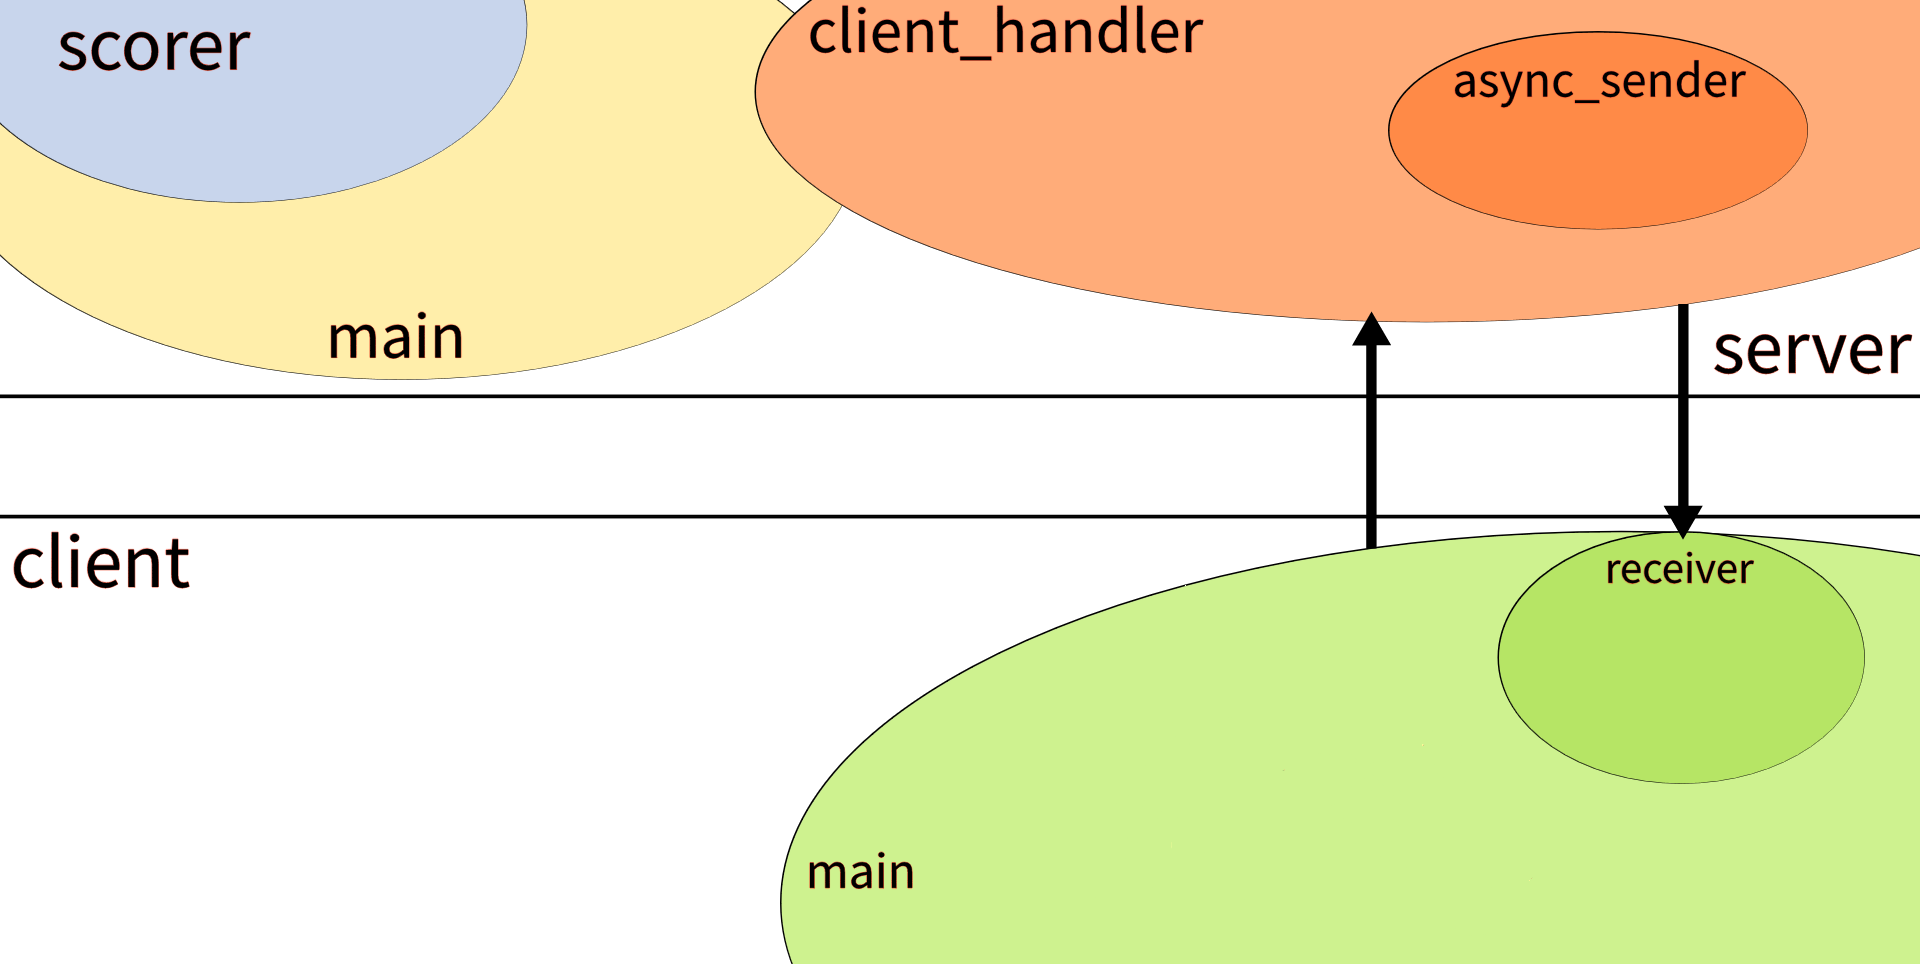
\includegraphics[keepaspectratio=true,scale=0.22]{scheme.png}
        Rappresentazione concettuale dei vari thread che compongono il client e il server
    \end{figure}
    
        \subsection{Client}
        Il client è composto di due thread diversi:
        \begin{itemize}
        \item \textbf{receiver}: il thread del receiver è responsabile di ricevere tutti i messaggi inviati dal server, sia asincroni che sincroni, interpretandoli un pezzo alla volta. Se è una risposta del server a un comando del client (tranne 'classifica', fare rif. Sezione 4) lo comunica al main, se invece riguarda la classifica finale se ne occupa personalmente. Inizia formattando il mesaggio CSV in un formato leggibile per l'utente e lo printa, svolgendo anche una tcflush dello \textbf{STDIN}. Questo viene fatto per pulire eventuali messaggi che l'utente stava digitando e che sarebbero stati interrotti dalla ricezione della classifica se ricevuta asincronamente.
        \item \textbf{main}: il thread principale inizia controllando i parametri con cui il programma è stato chiamato e tenta di stabilire una connessione. Una volta fatto, entra in un ciclo in cui legge i comandi dell'utente tramite \textbf{STDOUT}. Per ogni comando, gestisce immediatamente eventuali errori comunicandoli all'utente oppure inoltrando una richiesta al server se corretto. Attende poi risposta dal receiver e, in base al comando iniziale e alla risposta data dal server, fornisce un risultato all'utente. Il thread principale si occupa anche della gestione del \textbf{SIGINT} per garantire una chiusura completa e graceful dell'applicazione.
        \end{itemize}
        \subsection{Server}
        Il server è composto invece da 2 thread di base e 2 thread per ciascun client:
        \begin{itemize}
            \item \textbf{main}: il 'main' thread gestisce il controllo sui parametri obbligatori e opzionali, configurando le variabili per garantire un'esecuzione corretta. Dopodiché entra in attesa costante di nuove connessioni e, una volta ricevuta una, crea i thread dedicati alla gestione, esegue la \textbf{pthread\_detatch()} per impedire la creazione di zombie threads, aggiunge il player alla lista e ritorna in attesa.
            \item \textbf{scorer}: il thread 'scorer' gestisce il game loop. È responsabile della generazione della matrice, del controllo del timer di gioco/pausa, di richiedere l'invio dei punteggi sulla coda appositamente creata e successivamente di fornirli ai vari client. Questo è anche il thread che gestisce il segnale di \textbf{SIGINT} che potrebbe essere inviato. Quando questo segnale viene ricevuto, viene chiamata la funzione di \textbf{cleanup} che assicura una graceful closure, liberando tutta la memoria allocata dinamicamente.
            \item \textbf{clientHandler}: il thread del 'clientHandler' rimane in costante ascolto sul socket del client fino a quando lo user che gestisce non è impostato come inattivo. Una volta ricevuta una richiesta, la interpreta in base ai parametri impostati al momento (come lo stato della partita in corso o la disponibilità del nome utente richiesto durante la registrazione) e genera una risposta che, dopo aver assicurato la mutex sul socket, invia al client.
            \item \textbf{AsyncMsgSender}: questo thread gestisce tutto ciò che riguarda il messaggio di fine partita. Inizialmente, attende che lo scorer comunichi la fine della partita. Successivamente, se il giocatore è registrato e attivo, si aggiunge alla coda degli score. Dopo di ciò, attende che lo scorer abbia ricevuto tutti i punteggi e inviato il file CSV e, dopo aver assicurato l'accesso esclusivo al socket tramite mutex, invia il messaggio di classifica al client. Questo è anche il thread che gestisce l'\textbf{eliminazione del player}. Quando, a fine partita, si accorge che il player è stato impostato a inattivo, chiama una funzione di rimozione dell'utente dalla lista che si occupa anche della liberazione di trutta la memoria e delle variabili di sincronizzazione ed infine esce.
        \end{itemize}



    \clearpage
    \section{Scelte di progettazione}
    Le decisioni chiave prese nella progettazione si concentrano sulle strutture dati utilizzate sia dal client che dal server e dagli algoritmi fondamentali.
    \begin{itemize}
        \item \textbf{Matrice di gioco}: la matrice di gioco viene generata dal server durante ciascuna pausa e viene comunicata quando il client ne effettua richiesta tramite \textbf{MSG\_MATRICE}. Per gestire la presenza di "qu" ho utilizzato un carattere speciale '@' e questo mi permette di creare la matrice come un semplice char matrix[4][4]. Tuttavia, questo richiede alcuni passaggi in più per il "parsing" delle parole proposte, tenendo conto di quante volte appare "qu" nella parola proposta per assegnare i punti in maniera accurata ("qu" deve contare come 1 punto) e per printare correttamente la matrice a schermo. 

        Se viene richiesta la generazione casuale della matrice, utilizzo \textbf{srand(seed)} con quello fornito come parametro opzionale, oppure \textbf{srand(time(NULL))} se non specificato. 
        
        Se invece presa da un file, leggo l'intera riga e controllo se sono arrivato alla fine del file per un'eventuale rewind. Come richiesto dalla consegna, il server legge file del formato "A T L C I O Qu A D V E S I S B I\textbackslash n" (ovvero caratteri maiuscoli separati da spazi tranne per "Qu"). Questa sequenza viene poi convertita in lowercase prima di essere messa nella matrice, mantenendo questo formato per il resto del progetto. Ho scelto questa implementazione per rendere il formato visibile all'utente conforme a quello presente nel vocabolario (parole in lowercase), semplificando così lo sviluppo e la sottomissione delle parole per l'utente senza dover differenziare tra caratteri maiuscoli e "Qu" che è misto.\\
        Per la ricerca della parola nella matrice, la scorro tutta confrontando la prima lettera della parola con quella in matrice e, se trovo un match, effettuo una ricerca simil-DFS sfruttando una matrice di appoggio visited per tener traccia delle celle che ho già visitato.
        \item \textbf{Dizionario}: per la verifica delle parole ho optato per la struttura dati proposta della \textbf{Trie}. Ciasun nodo contiene la lettera che rappresenta, il numero di figli, un array dinamico di puntatori ai figli e un flag che indica se il nodo rappresenta la fine di una parola.
        
        Durante l'avvio del server, questo apre il file contenente il dizinario del formato specificato e inizia a leggere riga per riga popolando la Trie. In questo processo sfrutto le realloc dell'array dei figli per minimzzare il costo in memoria (18MB ca. per il file fornito) della struttura, riuscendo comunque a massimizzare l'efficienza della ricerca. Per questa infatti, data una parola lunga m caratteri, il costo è solo O(m) in quanto consiste solo nel cercare la lettera successiva tra i figli del nodo corrente.
        \item \textbf{Timer}: anche il timer di gioco/pausa è gestito come una struct. Questo contiene semplicemente un \textbf{time\_t} che rappresenta l'inizio del timer, la durata in secondi come int e una mutex per garantire l'accesso esclusivo. \\Il suo avvio prevede semplicemente di impostare il tempo di inizio a quello corrente del sistema e la durata. Per ottenere il tempo trascorso, basta una \textbf{diff\_time()} tra quello corrente e quello di avvio; da questo è poi facile ricavare il tempo rimanente. \\Ho preferito questo approccio a quello proposto della alarm, poiché la gestione dei segnali è più complessa e meno affidabile e ho notato che ridurla al minimo tende ad aumentare la robustezza del programma.
        \item \textbf{Player queue}: la player queue del server contiene tutte le informazioni necessario su ciascun giocatore. Composta da struct, questa mantiene dati cruciali per il corretto funzionamento e la sincronizzazione tra i thread che gestiscono il client.  
        \item \textbf{Score queue}: la score queue del server gestisce i punteggi finali prima che siano formattati in CSV e inviati ai client. Ogni gestore del client inserisce il proprio punteggio nella lista e, utilizzando una sorta di barriera, comunica quindi allo scorer che la coda è pronta per la generazione della stringa CSV.   
        \item \textbf{Protocollo di comunicazione}: come piccola aggiunta rispetto alla consegna, ho modificato i campi standard dei messaggi scambiati tra client e server da \textbf{[type, length, data]} a \textbf{[type, nLength, length, data]}. L'introduzione del campo nLength, seppur non necessario, facilita la ricezione dei messaggi, consentendo di determinare immediatamente quanti caratteri leggere per ottenere la lunghezza esatta del messaggio.
        \item \textbf{Server stdout}: Nonostante non fosse esplicitamente richiesto dalla consegna, ho introdotto alcuni messaggi inviati su \textbf{STDOUT} dal server. Questi messaggi forniscono una minima interfaccia per il debugging e l'errorchecking da parte dell'utente.
        \item \textbf{Connessione via sockets}: per stabilire la connessione via socket ho deciso di utilizzare \textbf{getaddrinfo()} per poter risolvere eventuali hostname presentati, rispetto ad alcune alternative che avevamo utilizzato durante il corso che funzionavano solo con indirizzi IP espliciti.
        \item \textbf{Nickname}: per il nickname dell'utente ho scelto di permettere un massimo di 12 caratteri, non escludendo alcun tipo di carattere. Naturalmente, non possono esserci due nickname identici nella stessa partita, a meno che tutti tranne uno si siano disconessi. Infatti, la disconnessione da una partita libera il nickname che l'utente stava utilizzando, permettendo ad un nuovo utente che si è unito di sceglierlo.
        \item \textbf{Comando classifica}: non essendo specificato nella consegna come il server dovesse gestire i messaggi di tipo \textbf{MSG\_PUNTI\_FINALI} ricevuti dal client, mi sono preso la libertà di aggiungere un comando \textbf{"classifica"} che il client puà utilizzare se registrato. Questo richiede al server la precedente classifica. Se disponibile, la printa nello stesso formato di quando è ricevuta asincronamente, altrimenti restituisce un'errore all'utente comunicando che al momento non è disponibile alcuna classifica.
    \end{itemize}


    
    \section{Testing}
    Come già affermato nella sezione 2, lo sviluppo è stato modulare e il testing si è svolto man mano che proseguivo con il progetto. Per garantire che il codice fosse affidabile ho utilizzato \textbf{CUnit}, una libreria open-source del C per svolgere test unitari. Per ciascun blocco sono stati quindi scritti dei test, progettati per verificare il corretto funzionamento delle librerie implementate. Questi sono stati poi eseguiti e verificati, garantendo che tutti gli eventuali errori potessero essere individuati e risolti. Questo mi ha permesso di isolare gli errori molto più semplicemente e di assicurarmi che, una volta combinati tutti i pezzi, avrei ottenuto un programma funzionante. 
    
    A causa della mole dei programmi finali, il testing via test unitari non è stato svolto direttamente sui file 'paroliere\_cl.c' e 'paroliere\_srv.c'. Tuttavia, questi file sono stati sottoposti a intensi test in vari ambienti di esecuzione, sia in scenari realistici (pochi utenti connessi) che complessi (con molti utenti che effettuano un elevato numero di richieste). Questo testing ha confermato l'affidabilità e la robustezza delle librerie sviluppate, assicurando che possano cooperare senza alcun errore e garantendo un elevato livello di affidabilità delle parti non di libreria che sono state aggiunte per portare a termine questo progetto.
    
    Per un debugging più rapido e occasionale, mi sono semplicemente avvalso di \textbf{gdb}, utilizzando il parametro -g in fase di compilazione. Con questo approccio sono riuscito comunque a individuare e risolvere piccoli problemi che insorgevano man mano che andavo avanti con lo sviluppo che però non giustificavano l'utilizzo di test unitari.
    
\end{document}